% Chapter 1

\chapter{Beam position monitor} % Main chapter title

\label{Chapter6} % For referencing the chapter elsewhere, use \ref{Chapter1} 
The serious systematic errors of the rotation and elastic deformation are from beam position.
We are developing Beam Position Monitor (BPM) for accurate measurement of beam position.
Previous study in LIGO have achieved 0.3~\% of uncertainty of the beam rotation effect by using Telephoto camera system (TCam).
They place the telephoto camera at 8~m far from the ETM. On the other hand, that of KAGRA is 36 m where is 4.5 times larger. Therefore, one of the most difficult technologies of calibration in KAGRA may be the beam position control.
We will demonstrate the system of the BPM as  the new technology. The BPM system is consists of QPD, Picomoter, and TCam

According to Eq.(\ref{eq:dx}), vector $\vec{a}$ and $\vec{b}$ corresponds to the rotation effect. $\vec{a}$ can be written as
\begin{equation}
\vec{a}=\vec{a_1} + \vec{a_2},
\end{equation}
where $\vec{a_1}$ and $\vec{a_2}$ are position vectors of two Pcal beams. We can measure the beam position of the main interferometer, $\vec{b}$, as well.
We can obtain the rotation term as
\begin{equation}
\frac{I}{M}\vec{a} \cdot \vec{b},
\end{equation}
where $I$ and $M$ are the inertial moment and mass of test mass.

Furthermore, the misaligned beam positions make the elastic deformation on the mirror surface due to asymmetry injection. It is one of the serious systematic errors.
Detail of the elastic deformation is described in Sec.~\ref{Chapter4}.

\section{Installation}
The installation phase of beam position monitor consists of two phases.
In first phase, we place the TCam system at the side of EXA and EYA chamber.
Detail of TCam is described in Sec.~\ref{Tcam_inst}. We connect the TCam and control PC (Raspberry pi) and operate it.
The purpose of TCam is not only calibration work but also other application.
We will monitor the pollution of water due to cryo-pumping effect. The taken picture will be analyzed automatically.
In second phase, we place the QPD and the pico motor for monitoring the beam drift. We will control the beam position using these components.
\section{Operation}
All the system is operated by MEDM system as shown in Fig.~\ref{fig:MEDM}.
For monitoring the beam positions, we use two pictures, which are with and without illuminator. We use the is Open Source Computer Vision Librarly (OpenCV) in python for image analysis, which is a library for open source computer vision developed and released by Intel.
The operation strategy is listed as follows:
\begin{enumerate}
 \item Take a JPAG style picture with illuminator. We set the integration time to 30 sec.
  \item Convert picture to gray scale using OpenCV.
  \item Set the reasonable threshold to find a boundary of the edge of ETM. 
   \item Mask the analysis region to separate the ETM edge and athers.
 \item Estimate the origin of the mirror coordinate by fitting of edge shape of the mirror.
 \item Turn off the illuminator and take picture with 30 sec integration time.
  \item Estimate the Pcal beam position and main interferometer position with no illumination picture. Then, we fit the gray scale picture using Gauss function.
   \item Make a picture overplotted the coordinate of Pcal and origin as shown in Fig.~\ref{fig:Beam_mon}.
   \end{enumerate}
   \begin{figure}
\begin{center}
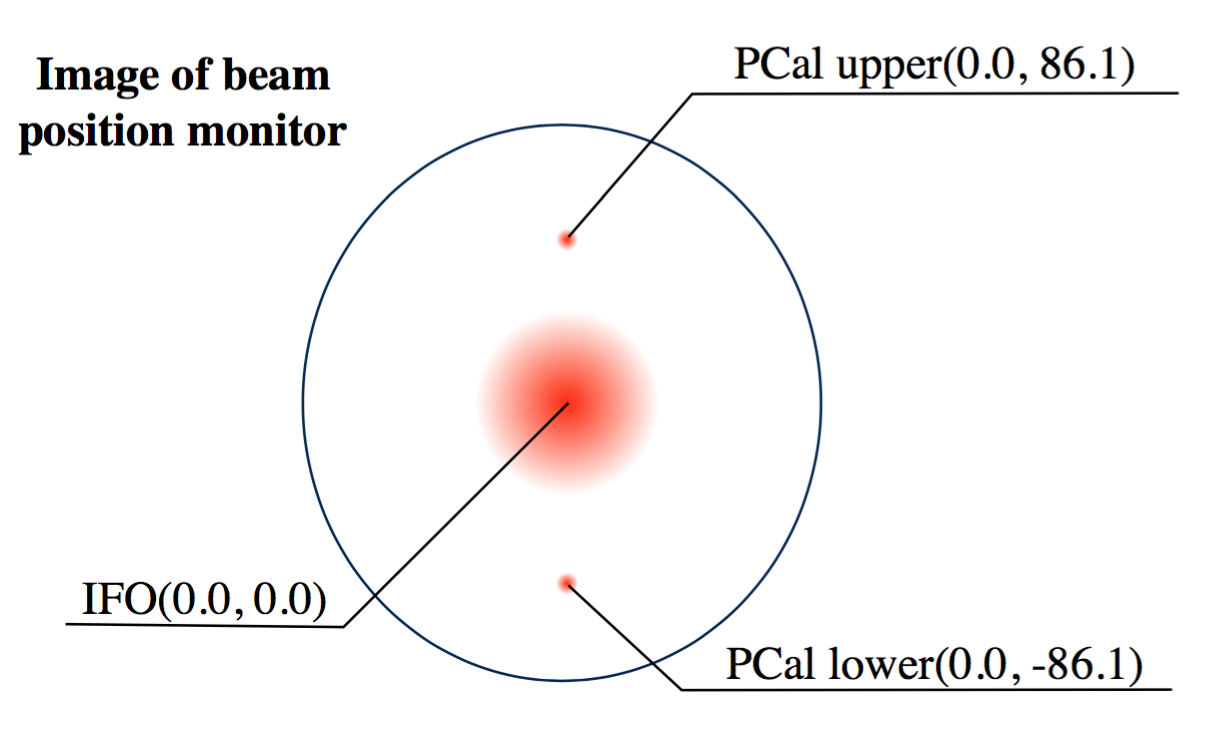
\includegraphics[width=14cm]{Figures/Beam_mon.eps}
\caption{Image of beam position monitor. We will over-plot the estimated beam position on the picture.} 
\label{fig:Beam_mon} 
\end{center}
\end{figure}


\section{Demonstration test}
We tried the demonstration test using TCam with 150mm diameter telescope and dummy target.
Figure~\ref{fig:Camera_test_setup} shows the test setup. 

   \begin{figure}
\begin{center}
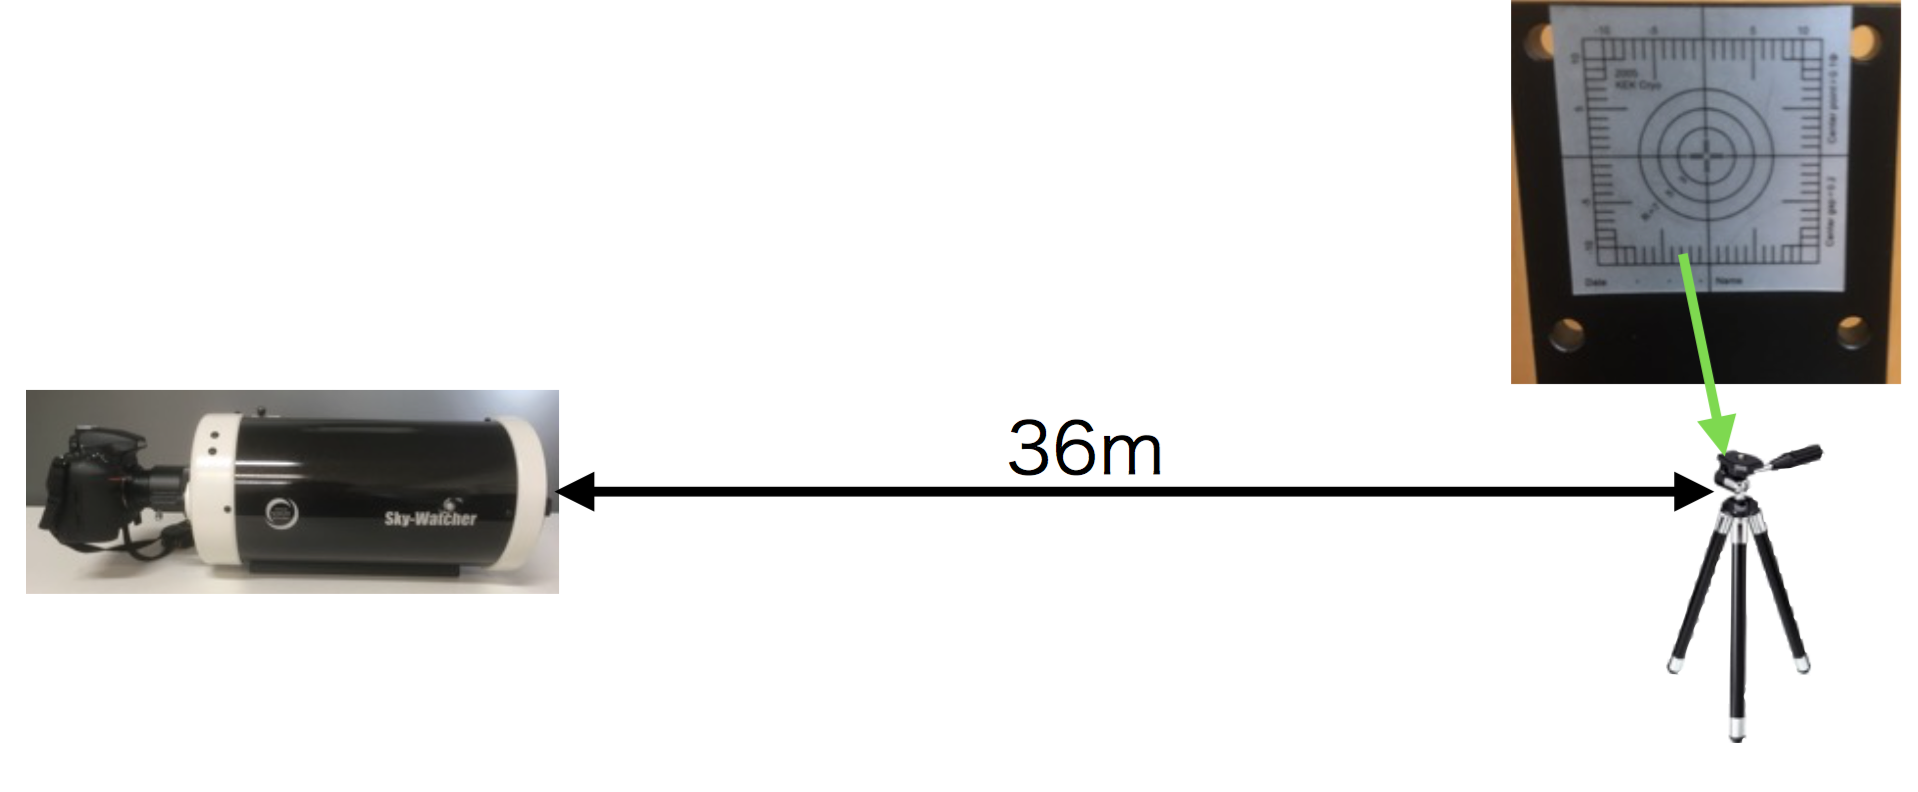
\includegraphics[width=14cm]{Figures/Camera_test_setup.eps}
\caption{Setup of demonstration test. We place the camera at 36m far from the ETM. This distance correspond to KAGRA configration.} 
\label{fig:Camera_test_setup} 
\end{center}
\end{figure}

We mount the target structure on the camera tripod. The size of target is $24 \times 24$~mm. Then, pixel size of this picture corresponds to $193 \times 193$. We can estimate the resolution per one pixel as $24~\mathrm{mm}/197~\mathrm{pix.}=0.12$~[mm/pix.]. The taken picture is shown in Fig.~\ref{fig:Camera_result}.
   \begin{figure}
\begin{center}
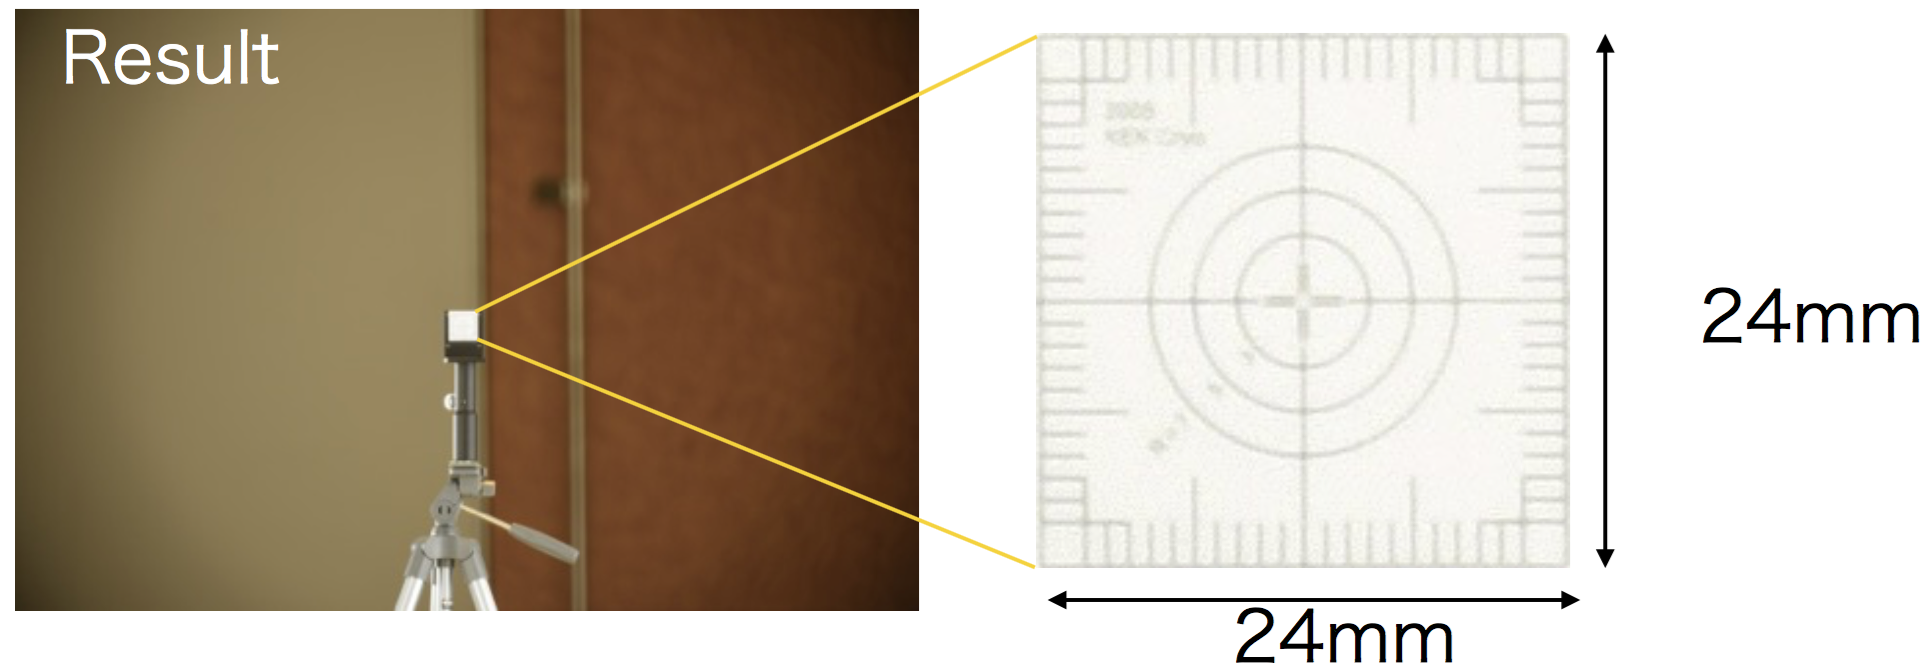
\includegraphics[width=14cm]{Figures/Camera_result.eps}
\caption{Raw data of Image analysis (left picture). We are trimming the target region. The size of target is $24 \times 24$~mm.} 
\label{fig:Camera_result} 
\end{center}
\end{figure}

We are trimming the target region. The trimmed data is converted to gray scale. We set the threshold point at 228.
Fig.~\ref{fig:Fitting_terget} shows the datas over the threshold.
We masked the data points.
The process of analysis is shown in Fig.~\ref{fig:Analysis_cam}.

   \begin{figure}
\begin{center}
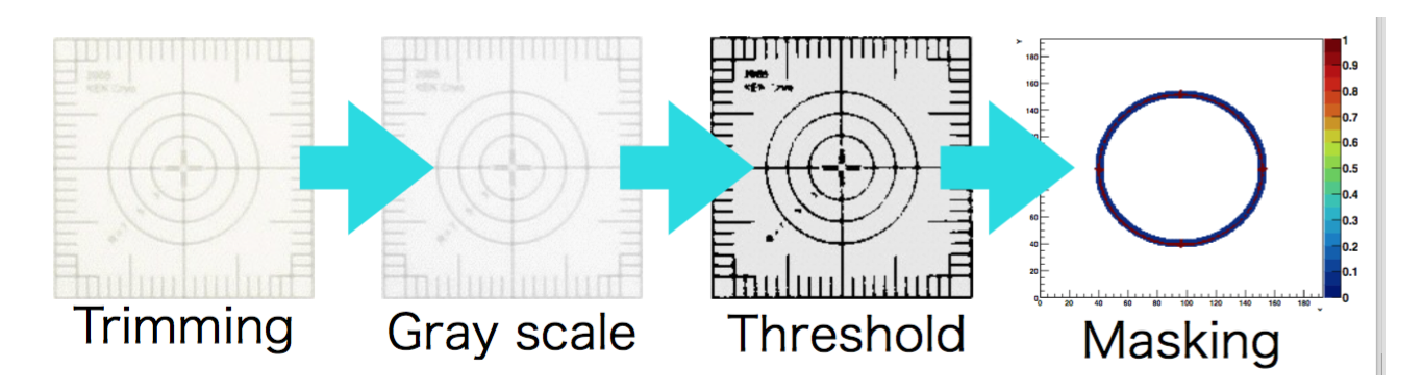
\includegraphics[width=14cm]{Figures/Analysis_cam.eps}
\caption{Strategy of analysis. First we trim the data around the target. Second we convert to Gray scale. Third we set the threshold. Fourth, we pick up the data point using mask. } 
\label{fig:Analysis_cam} 
\end{center}
\end{figure}

Finally, we have done a fitting and estimate the center point of the circle as shown in Fig.~\ref{fig:Fitting_target} and Table.~\ref{tab:Tcam_demo_fitting}.
Then, we assumed the following equation:
\begin{equation}
y=\sqrt{R^2-(x-x_0)^2}+y_0.
\end{equation} 
The measured and expected parameters are consistent within 1 sigma error.
Therefore, it imply that we can estimate the center point with $0.1$ mm resolution.
In the KAGRA, we use smaller telescope of 127 mm diameter.
We estimate the resolution when we use 127 mm telescope.
The estimated resolution is $24~\mathrm{mm}/193~\mathrm{pix.}\times 150~\mathrm{mm}/127~\mathrm{mm}=0.15$~[mm/pix.]. It meet our requirement.

   \begin{figure}
\begin{center}
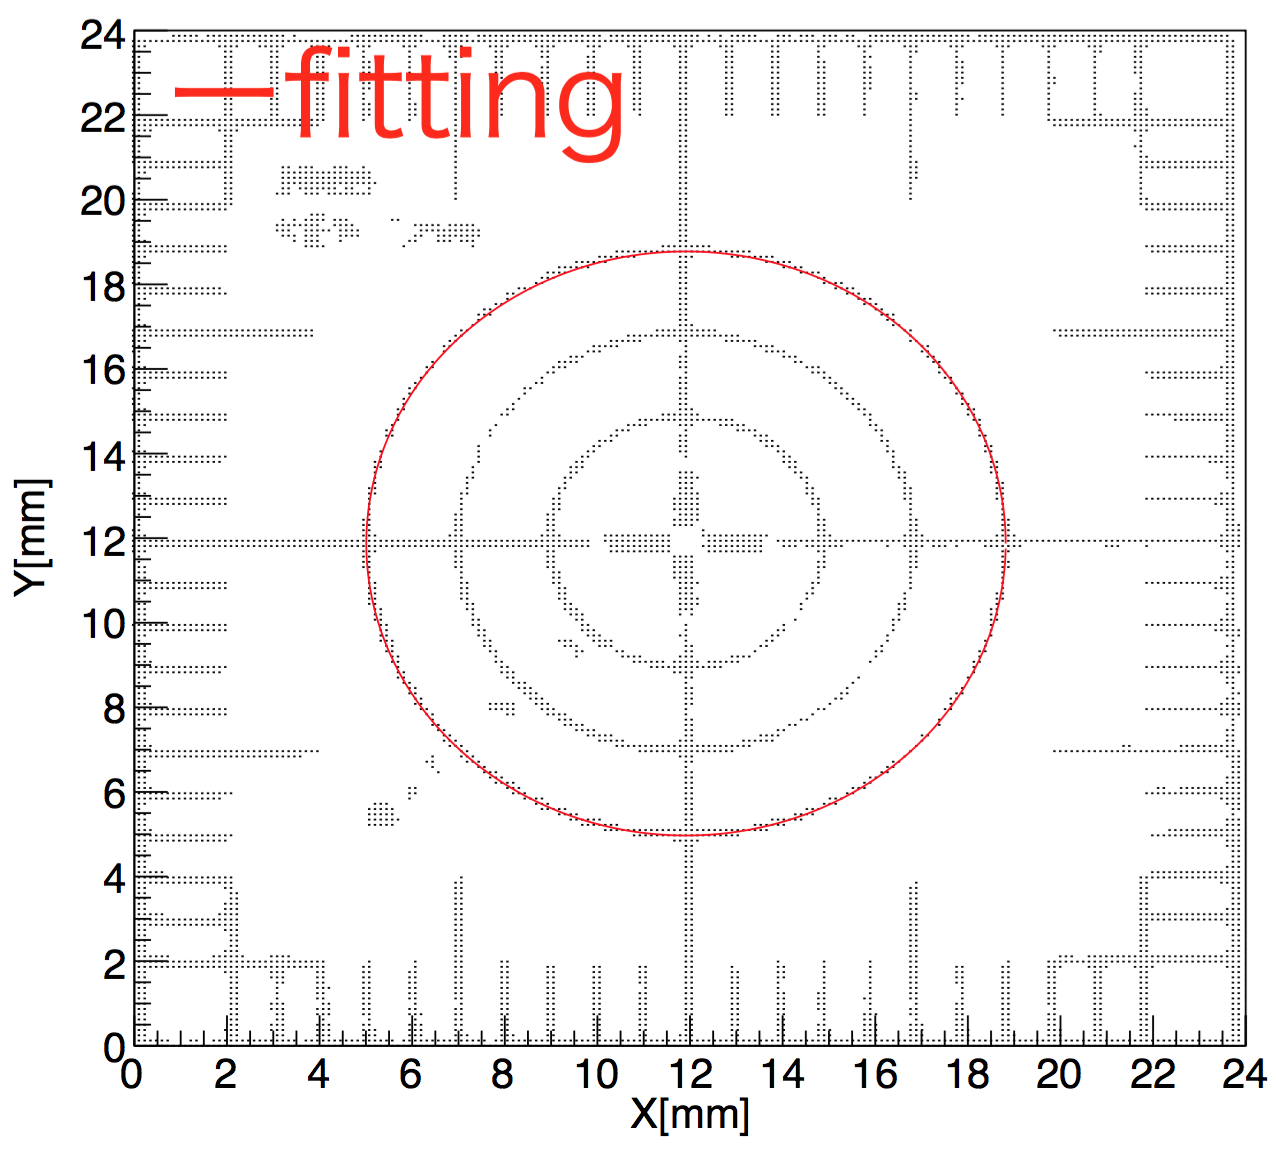
\includegraphics[width=14cm]{Figures/Fitting_target.eps}
\caption{Fitting result of image analysis. Black dots are data points larger than threshold. We masked data around outer circle. Red circle is best fitting.} 
\label{fig:Fitting_target} 
\end{center}
\end{figure}
   
 \begin{table}
\caption{Fitting result of camera demonstration test.}
\label{tab:Tcam_demo_fitting}
\centering
\begin{tabular}{ccc}
\toprule
\tabhead{Parameter} & \tabhead{Measured}& \tabhead{Expected}  \\
\midrule
R &$6.9\pm0.1$ mm& 7.0 mm \\
$x_0$ &$11.9\pm0.1$ mm& 12.0 mm \\
$y_0$&$11.9\pm0.1$ mm& 12.0 mm \\
\bottomrule\\
\end{tabular}
\end{table}

\section{Summary}
This chapter has considered the beam position monitor for KAGRA Pcal. The KAGRA photon calibrator is placed at 36 m far from the ETM. This number is larger than that of LIGO and VIRGO. Therefor, the beam position control technique is expected to play a essential role for reducing the systematic error. This system can be applied to LIGO or Virgo as well as KAGRA.

 